\documentclass[twoside,numberorder]{csbachelor}

%==============================================================
%==============================================================

\usepackage{url}
\usepackage{subfigure}

% 张海:其他引用
\usepackage[hidelinks]{hyperref}
\usepackage{pdfpages}

% 一些全局工具的定义
\DeclareMathOperator*{\argmin}{arg\,min}
\DeclareMathOperator*{\argmax}{arg\,max}

%==============================================================
%==============================================================

\begin{document}

\pagestyle{empty}

%==============================================================
%==============================================================

  % 论文题目:{中文}{英文}
  \zjutitle{在线交互式神经元重建的服务器系统}
           {todo}
  % 作者:{中文姓名}{英文}{学号}
  \zjuauthor{曲衡}{Heng Qu}{3130000569}
  % 指导教师:{导师中文名}{导师英文名}
  \zjumentor{郑能干}{Nenggan Zheng}
  % 个人信息:{年级}{专业名称}
  \zjuinfo{2013级}{计算机科学与技术}
  % 学院信息:{学院中文}{学院英文}
  \zjucollege{计算机科学与技术学院}{College of Computer Science and Technology}
  % 日期:{Submitted Date}
  %\zjudate{2017-03-29}

%==============================================================

  \thispagestyle{empty}

{
\setlength{\parindent}{0em}
\renewcommand{\baselinestretch}{2}

\vspace*{-7mm}

\begin{center}
  
\includegraphics[width=108mm]{data/cover/xiaoming}
\end{center}

\vspace{-1mm}

{
\renewcommand{\baselinestretch}{1.8}
\heiti\erhao\bfseries
\centering
本~~科~~生~~毕~~业~~设~~计 \\
中期报告 \par
}

\vspace{4em}

\begin{center}
  
\includegraphics[width=35mm]{data/cover/xiaobiao}
\end{center}

\vspace{3em}

{
\renewcommand{\baselinestretch}{1.65}
\songti\sanhao\bfseries
\centering
题目 \; \underline{\makebox[16em]{\zjutitlec}} \\
姓名 \; \underline{\makebox[16em]{\zjuauthornamec}} \\
学号 \; \underline{\makebox[16em]{\zjuauthorid}} \\
指导教师 \; \underline{\makebox[14em]{\zjumentorc}} \\
年级与专业 \; \underline{\makebox[13em]{\zjugrade~~\zjumajor}} \\
所在学院 \; \underline{\makebox[14em]{\zjucollegec}} \par
}
}

\ifthenelse{\equal{\zjuside}{T}}{\newpage\mbox{}\thispagestyle{empty}}{}


  \tableofcontents
  \thispagestyle{toc}
  %\chaptermark{目录}

  \mainmatter

  {
    \pagestyle{kaitibaogao}
    \makeatletter
      \let\ps@plain\ps@kaitibaogao
    \makeatother
    \chapter*{\zjutitlec 开题报告}

\section{项目背景}
将原始神经元图像信息进行神经元追踪和数字重建,有助于神经科学家直观地观察神经元结构,理解大脑运作的原理,甚至于探索智能的起源。因此,对大脑神经元相互连接形成的复杂网络进行数字重建一直是大脑神经科学家的目标之一。最近在神经元拓扑结构的自动化数字重建算法上取得了一些进展,如 Cannon RC 等人在海马神经重建上做出的工作\cite{Cannon1998An},Feng L 等人使用 mGRASP 在鼠类大脑上进行的重建工作\cite{Druckmann2014Structured}均取得了出色的进展。

由于神经元拓扑结构的复杂性,在一些自动化重建结果的细节上仍然需要研究人员对数字重建的结果进行人工纠正和修改,以确保数字重建工作的准确性。另外研究人员需要对数字重建结果进行编辑,比如添加或删除一些网络分支等。为了便于研究人员编辑数字重建的结果,根据“所见即所得”的原则,设计出了 SWC 格式\cite{Peng2011Proof}。SWC 框架有以下特征: 清楚的 SWC 结构以及原始数据参考的可视化,明确定义的可操作单元,以及将用户输入和编辑操作直观地对应起来。在 SWC 格式的基础上,研究人员可以方便、直观地纠正自动化数字重建结果的错误,添加新的分支或删除已有分支。

尽管在 SWC 格式的基础上已经开发出了大量可以产生 SWC 格式文件的神经元结构重建软件,例如专注于半自动重建的 FARSIGHT \cite{Luisi2011The}、半手动半自动重建的 Neuromantic \cite{Myatt2012Neuromantic},以及一些其他主流数字重建工具 Vaa3D \cite{Peng2010Seeing}、Neurostudio \cite{Rodriguez2006Rayburst} 等等。但是这些软件并没有充分利用 SWC 格式的优点,并且为用户提供高效、精确重建的界面,在 \cite{Feng2014neuTube} 中对这些软件的优缺点进行了详细的论述。为了充分发挥 SWC 格式高效,精确的优点,提供一个学习成本低,操作直观,并能提供相应的数据可视化功能,赵挺老师基于 SWC 格式,设计了名为 neuTube 的新软件\cite{Feng2014neuTube},同时具备 2D 和 3D 的可视化和直观的编辑、绘制功能。

由于 neuTube 是运行在单机的软件,无法满足多用户协同编辑修改的需求,也不利于数字重建结果的交流,无法共享完成数字重建的神经元结构。随着计算机性能和网速的提升,使得在线实时编辑神经元网络结构成为了可能。在此背景下,我们希望设计并实现一个在线多用户的神经元网络结构编辑平台,利用互联网便于数据共享的特点,帮助神经学研究人员便捷地进行异地,多用户协同编辑神经元网络结构,并能分享完成数字重建的神经元结构,共同探索神经元结构下的奥秘。

\section{目标和任务}
\subsection{目标}
我们的目标是设计并实现在线多用户的神经元网络结构编辑平台,利用互联网数据共享的特点,帮助神经学研究人员可以进行异地,多用户协同编辑神经网络结构,并能分享人工纠正、修改得到的神经元结构。充分发挥 SWC 文件格式准确,清楚,高效的优势,提供一个便于交互,同时具备 2D 和 3D 的可视化和直观的编辑、绘制功能的在线多用户神经网络结构编辑平台,并能处理多用户同时编辑时可能产生的冲突。

在这个平台上,用户可以上传神经回路的原始图像信息并储存在云端的服务器之中,利用 neuTube 或自己实现神经元网络结构的自动化数字重建工作。使用 SWC 格式储存数字重建工作的结果,作为后续修改、编辑的基础。平台包含数据可视化的功能,将数字重建结果以 2D 和 3D 的形式展现给用户。用户可以对数字重建结果进行人工编辑、修改,纠正自动数字重建结果中不精确的细节。用户也可以在已经完成的数字重建结果的基础上,删除已有分支或添加新的分支。

由于允许多用户同时编辑同一份 SWC 文件,这可能会造成文件内容的冲突。我们需要提供一套文件冲突解决方案,在文件内容产生冲突的时候尽可能地自动解决冲突,并能将实在解决不了的冲突准确、直观的表述给用户,便于用户手动解决冲突。

\subsection{任务}
设计完成上述需求的神经元网络结构编辑平台,将原始神经元图像信息应用于本平台,由神经科学家通过本平台编辑,修改完成数字重建的神经元结构,并根据反馈提高平台的可用性。
对系统的要求:

1. 交换界面简洁明了,操作简洁高效

2. 对多用户协同编辑提供支持

3. 能够解决多用户协同编辑产生的冲突

4. 用户操作延迟较低,没有明显的卡顿

\section{可行性分析}
郑能干老师和赵挺老师作为指导老师,在神经网络结构重建与编辑领域具有多年的工作经验,提供了清晰、明确的工作方向,在可能遇到问题的地方提供指导和帮助,为解决潜在的问题提供了保障。neuTube 作为已经实现的单机版本,明确了项目需求,展示出一些可能存在的问题,使我对该项目的理解更加深入透彻。技术方案里面涉及的很多技术是由赵挺老师所在实验室开发的,甚至是由赵挺老师本人编写完成的。两位指导老师提供的技术指导大大提高了项目可行性。

项目组积累了大量原始神经元切片图像数据,有充分的测试数据完成平台设计与开发。

项目前期对项目可能涉及到的技术做了充分的研究,尝试,对顺利完成项目内容,达成项目目标有充分的信心。

由于本项目不涉及硬件方面,项目经费需求较小。项目涉及到的服务器和开发平台均能利用现有实验室资源完成,可行性较高。

\section{初步技术方案和关键技术考虑}
技术方案涉及原始图像信息储存与数字重建结果储存,用户数据信息储存,网络应用开发以及前端可视化展示,共4个部分。

\subsection{原始图像信息与数字重建结果储存}
我们初步计划采用 DVID 储存原始图像信息与数字重建结果。DVID 是一个分布式面向图像的数据服务,主要用于图像分析与可视化。DVID 有如下特点:

1. 便于扩展数据类型,允许用户根据数据特点加速访问速度,减少储存空间,提供方便的 API。这为储存数字重建结果提供了便利。

2. 为分布式数据储存提供了类似于 GIT 的版本控制系统,在此基础之上我们可以解决多用户同时编辑产生冲突的问题。

3. 方便连接其他 API 如 Google BrainMaps 和 OpenConnectome 等。

4. 支持多分辨率图像数据,使得用户可以在不同尺度下观察图像信息。

在 DVID 的基础上,可以构建出多用户的原始图像信息与数字重建结果储存仓库,将数据储存抽象成数据存储服务,便于专注于完成核心算法和逻辑。

\subsection{用户数据信息储存}
初步计划采用 PostgreSQL 数据库储存用户信息。PostgreSQL 最初由加州大学伯克利分校计算机系开发完成。在支持大部分 SQL 标准之上,提供了许多诸如复杂查询,多版本并行控制,事物完整性等现代特性。由于 PostreSQL 对标准 SQL 支持度较高,可以方便的和 DVID 联系起来,将用户信息和原始图像信息,数字重建结果对应起来。利用 PostgreSQL 支持的储存过程,事物以及多版本并行控制特性,我们可以方便的实现分布式,多用户实时编辑平台,并解决多用户同时编辑可能产生冲突的问题。

\subsection{网络应用开发}
初步计划采用 Node.js 和 Express 完成网络应用开发。
Node.js 是一个基于 Chrome V8 引起的 JavaScript 的运行环境。Node.js 使用了一个事件驱动、非阻塞式 I/O 的模型,使其轻量又高效。Express 是一个基于 Node.js 平台的极简、灵活的 web 应用开发框架,提供丰富的 HTTP 快捷方式和任意排列组合的 Connect 中间件,帮助快速、简单的创建健壮、友好的 API。
\begin{figure}
\centering
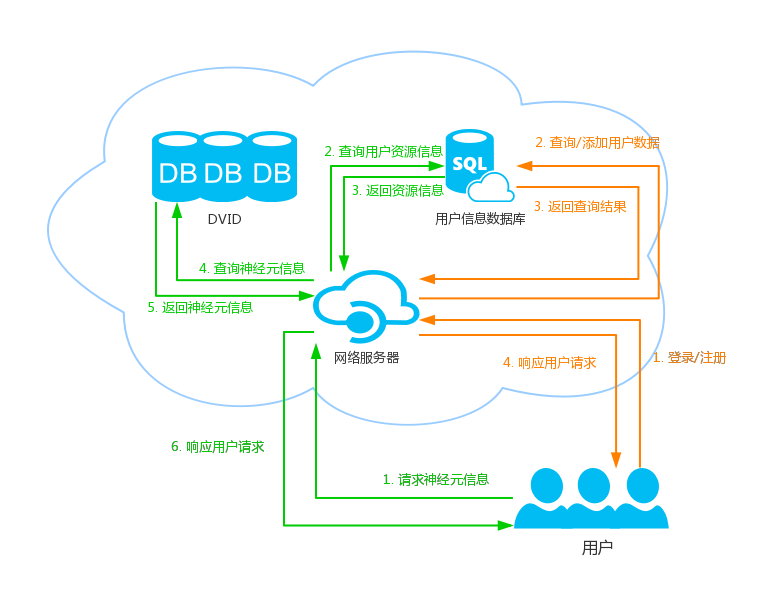
\includegraphics[width=108mm]{images/server}
\caption{分布式计算服务结构}
\label{server}
\end{figure}
基于这两个工具,可以方便快速的搭建一个无状态的服务器,初步设计出一个分布式计算服务结构如图 \ref{server} 所示,便于针对用户数量以及数据请求量进行扩展。搭配之前采用的分布式数据库,网络应用平台的可扩展性较高,可以用来应对多用户同时编辑大数据量的数据,并提供相应可视化算法所需的计算服务的应用场景。

\subsection{前端可视化展示}
这部分工作主要由同组其他同学完成,主要用到的技术有 Three.js 和 React 等, 这里不再赘述。 

\section{预期工作结果}
1. 神经元结构编辑平台

设计并实现一个同时具备 2D 和 3D 的可视化界面,为用户提供直观的编辑、绘制功能,支持多用户同时在线并可以协同编辑的神经元结构平台。实验室其他同学完成数据可视化工作,我主要实现平台的后端支持。

2. 同时在线用户数测试报告

对神经元结构编辑平台进行压力测试,根据测试结果进行性能调优,使之支持尽可能多的同时在线用户数量(数千用户同时在线,取决于平台后端计算机的性能和数量)。完成性能调优后提供一份完整的性能测试报告。

3. 用户操作延迟测试报告

对前端可视化操作的响应时间进行压力测试,根据测试结果进行性能调优,使用户操作的响应时间在毫秒级别(大量数据的上传时间取决去客户端所处网络环境)。对各个操作的响应时间及优化结果提供详细的测试报告。


\section{进度计划}

本项目的整体计划如下表所示:

\begin{table}[!htbp]
\centering
\begin{tabular}{|l|l|}
\hline
时间 & 主要工作 \\ \hline
2017 年 3 月 1 日 至 3 月 15 日& 完成项目功能点的需求及初步技术方案设计 \\ \hline
2017 年 3 月 16 日 至 3 月 29 日& 完成多用户平台设计 \\ \hline
2017 年 4 月 1 日 至 4 月 15 日& 初步完成需求的功能点 \\ \hline
2017 年 4 月 16 日 至 4 月 30 日& 并根据指导老师意见进行功能迭代,开始撰写论文 \\ \hline
2017 年 5 月 1 日 至 5 月 30 日& 根据测试结果进行性能调优,根据老师意见修改并完成论文 \\ \hline

\end{tabular}
\caption{项目进度计划}
\label{table:schedule}
\end{table}

\bibliographystyle{data/gbt7714-2005}
{
\renewcommand{\chapter}[2]{\section*{#2}\addcontentsline{toc}{section}{#2}}
\bibliography{data/kaitibaogao}
}

% 按文章长度需要启用
\ifthenelse{\equal{\zjuside}{T}}{\newpage\mbox{}\thispagestyle{empty}}{}

  }

\end{document}
